\section{Background on OpenWSN}
\label{sec:background-openwsn}


\begin{figure*}[!htb]
\centering
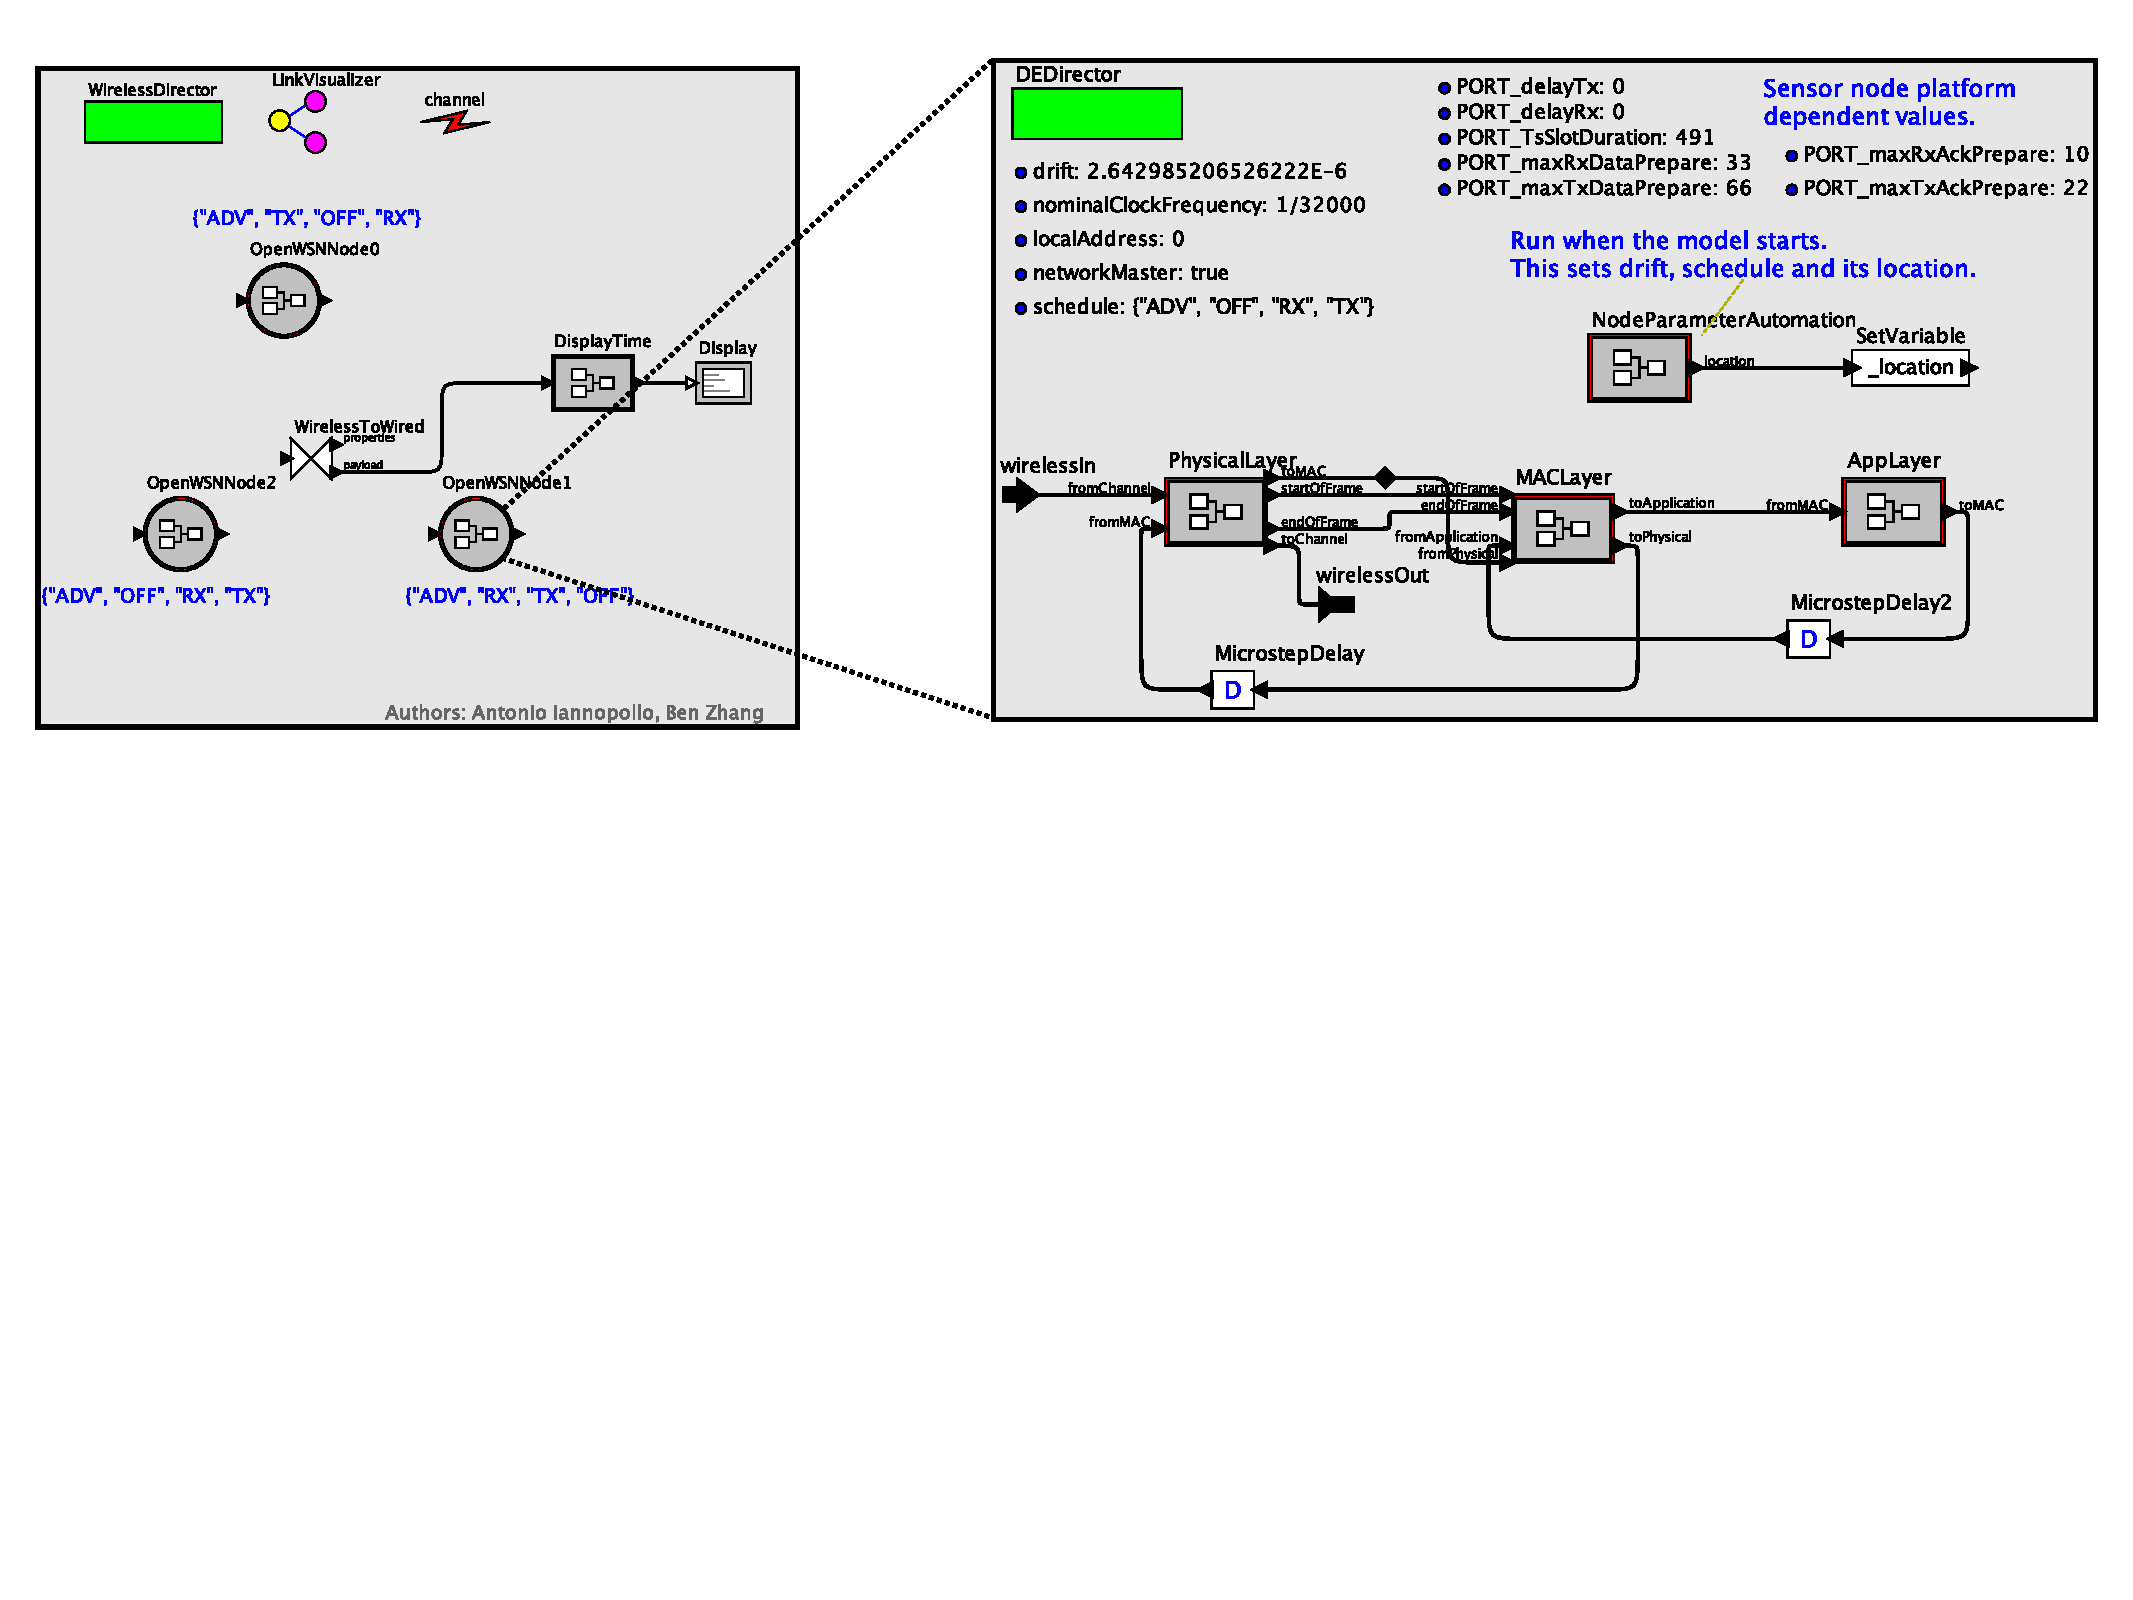
\includegraphics[width=1\textwidth]{figures/PaperOpenWSNNode}
\caption{An example application of three nodes ({\em left}) and the simplified network stack ({\em right}).}
\label{fig:OpenWSNNode}
\end{figure*}

In this section, we provide a brief overview of the OpenWSN protocol stack. Interested readers can read \cite{watteyne2012openwsn, IEEE802.15.4e} and visit OpenWSN website\footnote{\label{note:openWSN}https://openwsn.atlassian.net/wiki/} for more information. 

{\bf Slotframe:} IEEE802.15.4e defines a {\em slotframe} structure. A slotframe is a group of temporal slots which is repeated over time. Current OpenWSN implementation uses 15ms slots. A {\em schedule} tells the node whether it should transmit, receive or sleep in a particular slot. The construction of such schedule if out of the scope of IEEE802.15.4e.

{\bf Time Synchronization:} When a node joins a network, it aligns its slot boundary with other nodes (slot synchronization) and set its Absolute Slot Number (ASN) to the network ASN (ASN synchronization). In this way, all nodes will enter in a new slot at the same time (following their pre-defined schedule). 

{\bf Re-synchronization:} Since the clock on the embedded platforms is not perfect (typical clock drift is around 10 parts-per-million (ppm)), a re-synchronization mechanism is needed. OpenWSN performs re-synchronization whenever a packet transmission happens. Each node picks as reference the neighbor that is closer to the root of the network as its time master, and the synchronization is achieved by aligning its next slot boundary to the master's. When there is no packet transmission, a {\em KeepAlive} packet is generated (every 30 seconds is a typical value).

{\bf OpenWSN State Machine:} In each slot, given the schedule, the node behaves according to a state machine. This state machine defines how the synchronization is reached and maintained, as well as transmission and reception. We defer the discussion here because this will be the main focus of our modeling work described in the next section.

{\bf Packet format:} the OpenWSN stack defines several types of packet. In our work, we consider three of them, related to the MAC layer: \texttt{ADV}, \texttt{DATA}, \texttt{ACK}. The advertisement packet \texttt{ADV} is used to broadcast the network information (such as ASN) such that new node can join the network. The \texttt{DATA} packet encapsulates the upper layer payload. The \texttt{ACK} packet is used to acknowledge a data packet. It also contains time correction information such that the other node can perform re-synchronization (if needed).


%%% Local Variables: 
%%% mode: latex
%%% TeX-master: "ee219d"
%%% End: 
